Diagram 1 in Fig.~\ref{fig:diagrams} represents a second-order contribution to the energy and a so-called $2p-2h$ contribution to the intermediate states.
Write down the expression for the wave operator in this case and compare the possible contributions with the configuration interaction calculations of exercise 3). % chktex 10 % tex-fmt: skip
Comment your results for various values of $g \in [-1,1]$.

\subsection{}
For a second-order contribution to the energy, we get a contribution from the first-order wave operator, which is given by
% The first order wave operator is given by
\begin{align*}
    \vert \Psi^{(1)} \rangle
    = \frac{\hat{Q}}{\mathcal{E}_0 - \hat{H}_0} \hat{V} \vert \Phi_0 \rangle
    &= \frac{1}{4} \sum_{\substack{ab \\ ij}} \frac{\langle ab \vert V \vert ij \rangle}{\varepsilon_i + \varepsilon_j - \varepsilon_a - \varepsilon_b} \vert \Phi_{ij}^{ab} \rangle \\
    &= \frac{1}{8} \sum_{ai} \frac{\langle i\bar{i} \vert V \vert a\bar{a} \rangle}{i - a} \vert \Phi_{i\bar{i}}^{a\bar{a}} \rangle \\ % chktex 7
    &= -\frac{1}{4} \sum_{ai} \frac{g}{i - a} \vert \Phi_{i\bar{i}}^{a\bar{a}} \rangle, % chktex 7
\end{align*}
where we've again reduced the sum to just sum over the energy levels, and introduced a factor of 2 per spin state.
Here we are interested in each coefficient
\begin{equation*}
    \frac{g}{4(i - a)} \vert \Phi_{i\bar{i}}^{a\bar{a}} \rangle,
\end{equation*}
which we can compare with those found from the CI calculations.
The coefficients of the wave operator $\Psi^{(1)}$ are shown in Fig.~\ref{fig:f_coefficients}.

\begin{figure}
    \centering
    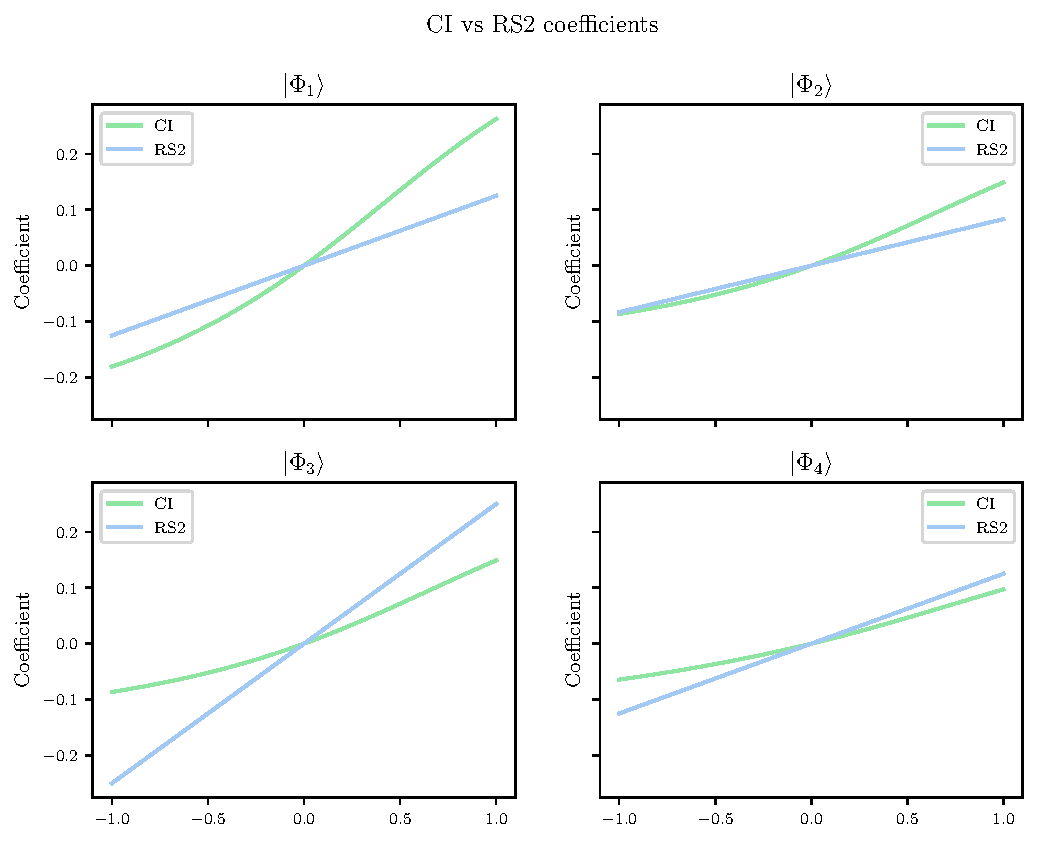
\includegraphics[width=\textwidth]{figures/f_coefficients.pdf}
    \caption{
        Coefficients of the wave operator $\Psi^{(1)}$ as a function of $g$, compared with those from the CI calculations.\label{fig:f_coefficients}
    }
\end{figure}

\begin{figure}[htbp]
    \centering
    \begin{subfigure}[b]{0.45\textwidth}
        \centering
        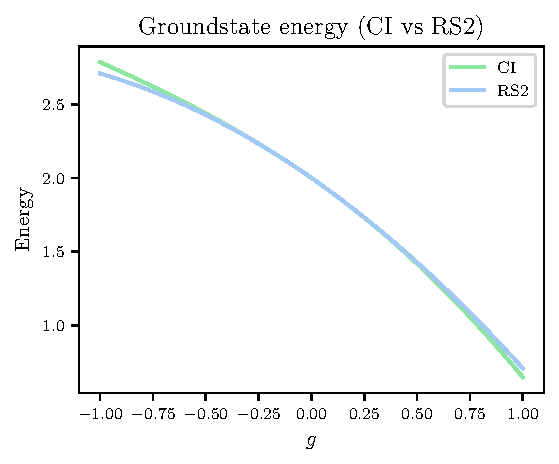
\includegraphics[width=\textwidth]{figures/f_groundstate_energy.pdf}
        \caption{
            Groundstate energy from RSPT.\label{fig:rs2_energy}
        }
    \end{subfigure}
    \hfill
    \begin{subfigure}[b]{0.48\textwidth}
        \centering
        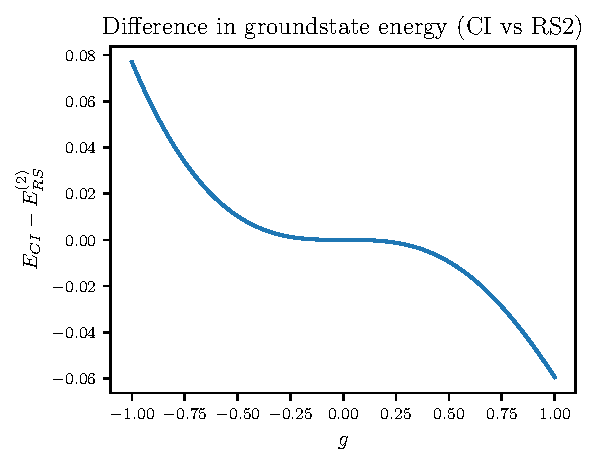
\includegraphics[width=\textwidth]{figures/f_groundstate_energy_diff.pdf}
        \caption{
            Difference in energy from RSPT.\label{fig:rs2_diff}
        }
    \end{subfigure}
    \caption{
        Groundstate energy from the Rayleigh-Schr\"odinger perturbation theory to second-order, compared with the CI results, as a function of $g$.\label{fig:rs2}
    }
\end{figure}

The second-order energy contribution is given by
\begin{align*}
    \langle \Phi_0 \vert \hat{V} \vert \Psi^{(1)} \rangle &= \frac{1}{4} \sum_{\substack{ab \\ ij}} \frac{\langle ab \vert V \vert ij \rangle}{\varepsilon_i + \varepsilon_j - \varepsilon_a - \varepsilon_b} \langle \Phi_0 \vert \hat{V} \vert \Phi_{ij}^{ab} \rangle \\
    &= \frac{1}{4} \sum_{\substack{ab \\ ij}} \frac{\langle ij \vert V \vert ab \rangle \langle ab \vert V \vert ij \rangle }{\varepsilon_i + \varepsilon_j - \varepsilon_a - \varepsilon_b} \\
    &= \frac{1}{4} \sum_{ai} \frac{
        \langle i\bar{i} \vert V \vert a\bar{a} \rangle % chktex 7
        \langle a\bar{a} \vert V \vert i\bar{i} \rangle % chktex 7
    }{2(\varepsilon_i - \varepsilon_a)}
\end{align*}
Changing the summation to just sum over the energy levels, we again need to introduce a factor of 2 per spin state, giving
\begin{equation*}
    \frac{1}{2} \sum_{ai} \frac{
        \langle i\bar{i} \vert V \vert a\bar{a} \rangle % chktex 7
        \langle a\bar{a} \vert V \vert i\bar{i} \rangle % chktex 7
    }{i - a} = \frac{1}{8} \sum_{ai} \frac{g^2}{i - a} = -\frac{7}{24} g^2
\end{equation*}
We thus get a total contribution with RSPT to second order of
\begin{equation*}
    2 - g - \frac{7}{24} g^2.
\end{equation*}

As we see in Fig.~\ref{fig:rs2}, the RSPT calculations serve as a good approximation for $g$ close to $0$, but differs both from above and below for larger values of $|g|$.
